\documentclass{beamer}
\usetheme{default}
\usecolortheme{seahorse}
\usepackage[utf8]{inputenc}
\usepackage{graphicx}
\usepackage{booktabs}
\usepackage{amsmath}
\usepackage{natbib}
\usepackage[english]{babel}
\usepackage{hyphenat}
\usepackage{tikz}
\usetikzlibrary{shapes,arrows.meta,positioning}

\title[Lecture 2]{The Questionnaire}
\subtitle{Advanced Master in Agricultural Economics and Policy}
\author{Giovanbattista Califano}
\date[Portici, 23/04/2026]{Attitudinal Scales for the Study \\ of Consumer Preferences \\ April 23, 2026}
\institute[UNINA]{University of Naples Federico II, giovanbattista.califano@unina.it}

\AtBeginSection[]
{
  \begin{frame}<beamer>
    \frametitle{Moving on to...}
    \tableofcontents[currentsection]
  \end{frame}
}

\begin{document}

\frame{\titlepage}

\begin{frame}{Roadmap}
    \begin{center}
        \begin{tabular}{|l|l|c|}
        \hline
        20/04 &  Hello, Psychometrics! & $\checkmark$ \\
        \hline
        23/04 &  The Questionnaire & $\bigcirc$ \\
        \hline
        24/04 & Reliability and Validity of a Measure & $\bigcirc$ \\
        \hline
        27/04 & Latent Variables: Reflective or Formative? & $\bigcirc$ \\
        \hline
        30/04 & A Bit of SEM & $\bigcirc$ \\
        \hline
        07/05 & Stata Stata Stata Stata Stata Stata Stata & $\bigcirc$ \\
        \hline
        \end{tabular}
    \end{center}
\vspace{0.1cm}
\footnotesize
Recommended readings: \\
\begin{itemize}
    \item Chapters 4 and 7 from \cite{jhangiani2019research}
    \item Chapters 7, 10 and 14 from \cite{olivero2022psicologia}
    \item Chapter 12 from \cite{mehmetoglu2022applied}
\end{itemize}
\scriptsize
\bibliographystyle{apalike}
\bibliography{text}
\end{frame}

\section{The Questionnaire}
\begin{frame}{A second Copernican revolution?}
\huge
    \[
      \Delta x \cdot \Delta p_x \;\ge\; \frac{\hbar}{2}
    \]
\end{frame}

\begin{frame}{A second Copernican revolution?}
    \[
      \Delta x \cdot \Delta p_x \;\ge\; \frac{\hbar}{2}
    \]
\begin{block}{Uncertainty Principle}
\small
    Stated by \textbf{Werner Heisenberg} in 1927, it represents a cornerstone of quantum mechanics and marked a radical break from the laws of classical mechanics. \\
    \smallskip
    We cannot know with absolute precision, simultaneously, both the position and the velocity of a particle: \textbf{the very act of measuring something changes it}. This is not a problem of imperfect instruments, but a fundamental characteristic of quantum nature.
\end{block}
\end{frame}

\begin{frame}{The questionnaire}
    The questionnaire is a \textbf{self-report} instrument used to collect quantitative and/or qualitative information. Since it is generally completed independently by the participant, it may create the impression that the researcher is external to the process; in reality, the researcher is solely responsible for the \\
    \vspace{1em}
    \pause
    \huge\centering
    \alert{DATA GENERATING PROCESS}
\end{frame}

\begin{frame}{The questionnaire}
\begin{block}{The participant}
    is not a database from which to extract data, but an \textbf{active subject} who uses various \textbf{contextual factors}, beyond the content of the questions, to make sense of the questionnaire they are filling in. Some contextual effects: \\
    \begin{itemize}
        \item The way the questionnaire is presented.
        \item The identity of the researcher and the research institution.
        \item The response alternatives.
        \item The order of the questions.
    \end{itemize}
\end{block}
\end{frame}

\begin{frame}{Example: Order effect}
\textit{Strack et al. (1988) asked some university students both how satisfied they were with their life in general and how often they went on dates.} \\
\vspace{1em}
\centering
\begin{tabular}{l|lclc}
    \toprule
   Order 1 & Satisfaction & $\rightarrow$ & Dates & $r$ = -.12 \\
   \midrule
   \pause
   Order 2 & Dates & $\rightarrow$ & Satisfaction & $r$ = +.66 \\
   \bottomrule
\end{tabular}
\vspace{0.3cm}
\begin{block}{Possible solutions?}
\pause
\begin{itemize}
    \item \textbf{Separate} the questions in the questionnaire.
    \pause
    \item \textbf{Randomise} the presentation of questions.
    \pause
    \item \textbf{Do both}.
\end{itemize}
\end{block}
\end{frame}

\begin{frame}{Cognitive processes in responding to an item}
How many alcoholic drinks do you consume on a typical day? \\
\vspace{0.2cm}
\begin{tabular}{ll}
    $\bigcirc$ & Much more than average \\
    $\bigcirc$ & Somewhat more than average \\
    $\bigcirc$ & About average \\
    $\bigcirc$ & Somewhat less than average \\
    $\bigcirc$ & Much less than average \\
\end{tabular}
\vspace{1em}
\\ \textit{Even when we ask an apparently simple question, the response process can be complex, open to interpretations and manipulations.}
\end{frame}

\begin{frame}{Cognitive processes in responding to an item}
  \resizebox{\textwidth}{!}{%
    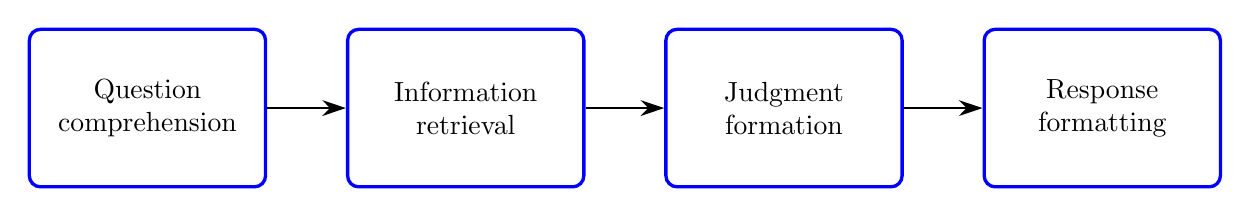
\begin{tikzpicture}[
      process/.style={
        rectangle,
        draw=blue, very thick,
        rounded corners,
        minimum width=3cm,
        minimum height=2cm,
        align=center
      },
      arrow/.style={
        -{Stealth[length=3mm,width=2mm]},
        thick
      }
    ]
      \node[process] (comprehension) {Question \\ comprehension};
      \node[process, right=of comprehension] (retrieval) {Information \\ retrieval};
      \node[process, right=of retrieval] (judgment) {Judgment \\ formation};
      \node[process, right=of judgment] (response) {Response \\ formatting};
      \draw[arrow] (comprehension) -- (retrieval);
      \draw[arrow] (retrieval) -- (judgment);
      \draw[arrow] (judgment) -- (response);
    \end{tikzpicture}%
  }
\end{frame}

\begin{frame}{The BORIS Model}
    The BORIS model\footnote{\scriptsize{Called BRUSO in \cite{jhangiani2019research}}} offers five useful principles for writing effective questionnaire questions.\\
    \vspace{1em}
    \begin{table}[]
        \centering
    \begin{tabular}{cc}
    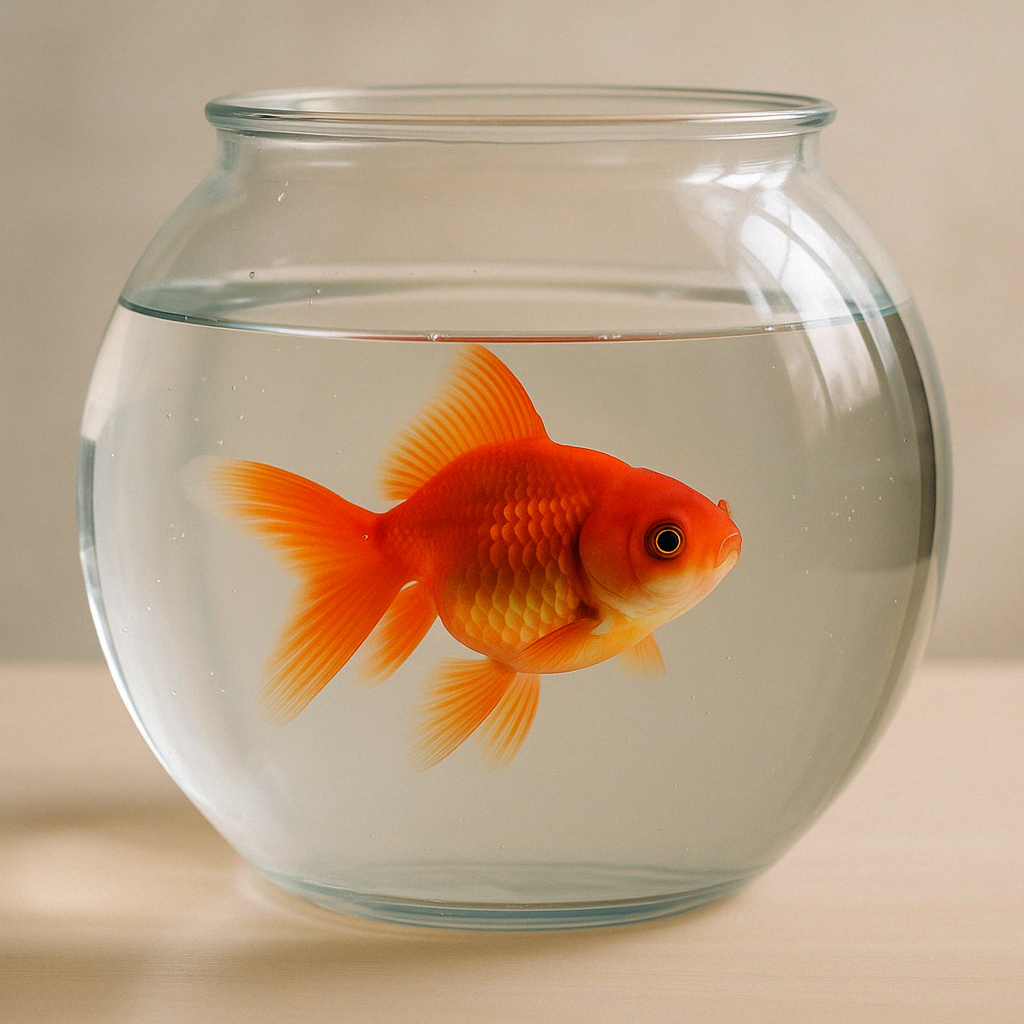
\includegraphics[width=0.45\linewidth]{boris.png} & 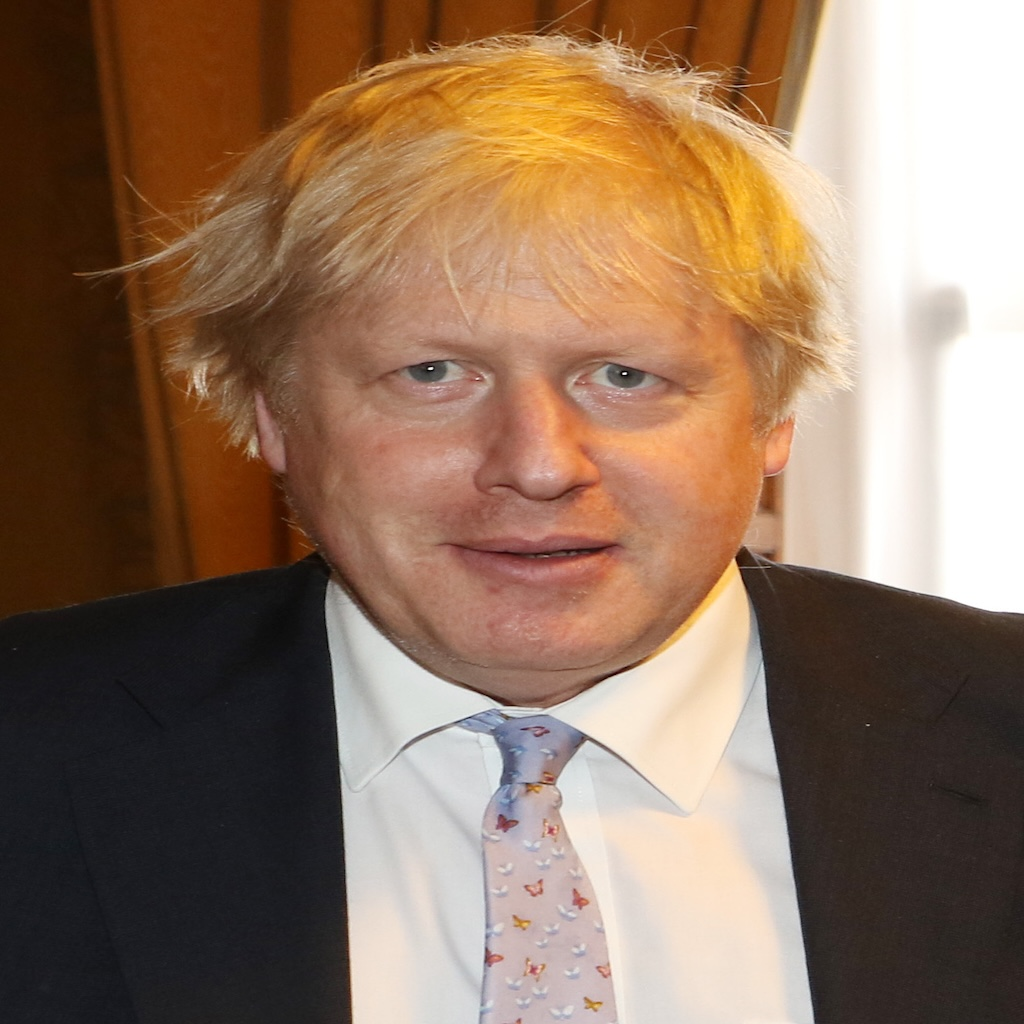
\includegraphics[width=0.45\linewidth]{boris2.jpg} \\
    \footnotesize{Goldfish} & \footnotesize{Former UK Prime Minister}
    \end{tabular}
    \end{table}
\end{frame}

\begin{frame}{The BORIS Model}
  \scriptsize
  \centering
  \begin{tabular}{lp{4cm}p{3.5cm}}
    \toprule
    \textbf{Criterion} & \textbf{Ineffective} & \textbf{OK} \\
    \midrule
    \textbf{B}revity & "Have you ever, at any point in your life, come across the concept of social agriculture?" & "Have you ever heard of social agriculture?" \\
    \\
    \textbf{O}bjectivity & "How much do you support the NoCap ethical certification?" & "What is your opinion on the NoCap certification?" \\
    \\
    \textbf{R}elevance & "Which party did you vote for in the last general election?" & Do not include the question if it is not clearly relevant. \\
    \\
    \textbf{I}nambiguity & "Would you consider yourself a health-conscious person?" & "Do you habitually check nutritional labels when shopping?" \\
    \\
    \textbf{S}pecificity & "Have you ever heard of integrated production and SQNPI?" & "Have you ever heard of integrated production?" \\
    \bottomrule
  \end{tabular}
\end{frame}

\section{What Attitudes Are and How to Measure Them}
\begin{frame}{Attitudes $\neq$ Aptitudes}
    \begin{block}{What are attitudes?}
        Since 1918 more than 500 definitions of attitudes have been coined! \\
        From the various definitions, a component of \textbf{evaluation} (positive–negative) of the subject with respect to an object emerges: \\
        \pause
        \small
    \begin{itemize}
        \item Allport (1954) defines attitude as a mental state, organised through experience, that exerts an influence on the individual's responses towards all objects and situations with which they are in relation.
        \item For Social Cognition (Fazio, 1986), an attitude is a cognitive structure constituted by the association in memory between the representation of the object and its evaluation.
        \item Mayers (2021) defines attitude as a favourable or unfavourable evaluation towards something or someone, often rooted in one's beliefs and exhibited in feelings and intentional behaviour.
    \end{itemize}
    \end{block}
\end{frame}

\begin{frame}{Attitudes $\neq$ Aptitudes}
    \begin{block}{What are attitudes for?}
        Katz (1960) suggests that attitudes can serve four main functions: \\
        \small
    \begin{enumerate}
        \item \textbf{Utilitarian}: the attitude towards a certain object develops to achieve a benefit or avoid a negative effect (e.g. positive attitude towards a vegan diet because it is perceived as healthier);
        \item \textbf{Value expression}: to express individual values and \textit{self-concept} (e.g. positive attitude towards a vegan diet to express one's \textit{ethical values});
        \item \textbf{Ego-defence}: to defend a perceived lack at the identity level (e.g. negative attitude towards a vegan diet, on the part of a man, because eating salad is seen as unmasculine);
        \item \textbf{Cognitive}: to respond to the need for order, balance and coherence...
    \end{enumerate}
    \end{block}
\end{frame}

\begin{frame}{Attitudes $\neq$ Aptitudes}
    \footnotesize
    \begin{block}{Balance Theory (Heider, 1946)}
        is grounded precisely in the principle of cognitive consistency, and posits the existence of triadic attitudinal structures that tend towards cognitive restructuring in case of imbalance. \\
        The triadic structure consists of at least two people and at most one object. Depending on the attitudes with which they are associated with one another, they can represent balanced or imbalanced structures that will therefore tend towards change. \\
        \vspace{0.5em}
        \centering
        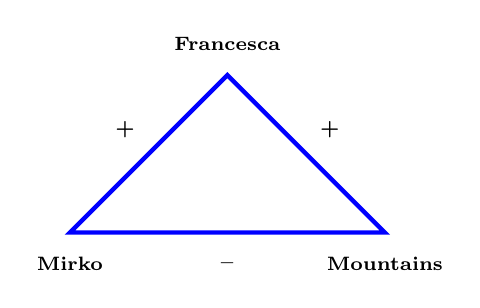
\begin{tikzpicture}
            \draw[blue, ultra thick] (4,0) -- (8,0) -- (6,2) -- cycle;
            \node at (4.7,1.3) {\textbf{\scriptsize+}};
            \node at (7.3,1.3) {\textbf{\scriptsize+}};
            \node at (6,-0.4) {\textbf{\scriptsize –}};
            \node at (4,-0.4) {\textbf{\scriptsize Mirko}};
            \node at (8,-0.4) {\textbf{\scriptsize Mountains}};
            \node at (6,2.4) {\textbf{\scriptsize Francesca}};
        \end{tikzpicture}
        \\
        \vspace{0.5em}
        \textit{\scriptsize A triad is considered balanced when the product of the signs is positive.} \\
    \end{block}
\end{frame}

\begin{frame}{Attitudes $\neq$ Aptitudes}
    \begin{block}{Balance Theory in marketing}
        Many companies use brand ambassadors beloved by the public to promote the formation of a positive attitude towards their product or service.  \\
        \vspace{0.5em}
        \centering
        \pause
        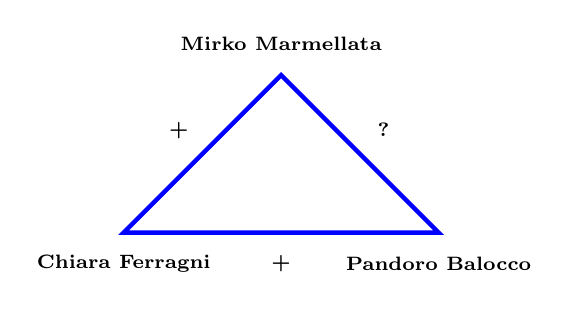
\begin{tikzpicture}
            \draw[blue, ultra thick] (4,0) -- (8,0) -- (6,2) -- cycle;
            \node at (4.7,1.3) {\textbf{\scriptsize +}};
            \node at (7.3,1.3) {\textbf{\scriptsize ?}};
            \node at (6,-0.4) {\textbf{\scriptsize +}};
            \node at (4,-0.4) {\textbf{\scriptsize Chiara Ferragni}};
            \node at (8,-0.4) {\textbf{\scriptsize Pandoro Balocco}};
            \node at (6,2.4) {\textbf{\scriptsize Mirko Marmellata}};
        \end{tikzpicture}
    \end{block}
\end{frame}

\begin{frame}{Attitudes $\neq$ Aptitudes}
    \begin{block}{Some basic characteristics:}
        \small
        \begin{itemize}
            \item Attitudes are relatively permanent over time and consistent across situations.
            \item Attitudes always imply a certain degree of abstraction and are generalisable to multiple situations, objects or conditions.
            \item Attitudes always have social relevance as they influence how a person relates to others, their preferences and their behaviours.
        \end{itemize}
        \textbf{Attitude is therefore a useful means of predicting consumer behaviour.}
    \end{block}
\end{frame}

\tikzset{
  block/.style = {draw=blue!80, fill=blue!10, very thick, ellipse, minimum height=2cm, minimum width=3cm, align=center}, arrow/.style = {thick, ->, >=Stealth}
}

\begin{frame}{Theory of Reasoned Action (Fishbein \& Ajzen, 1975)}
\resizebox{\textwidth}{!}{%
\centering
\begin{tikzpicture}[node distance=1.5cm, auto]
  \node[] (pbc) {};
  \node[block, above=of pbc] (att) {Attitude \\ towards the \\ behaviour};
  \node[block, below=of pbc] (ns) {Subjective norms};
  \node[block, right=of pbc] (int) {Behavioural \\ intention};
  \node[block, right=of int] (beh) {Behaviour};
  \draw[arrow] (att) -- (int);
  \draw[arrow] (ns)  -- (int);
  \draw[arrow] (int) -- (beh);
\end{tikzpicture}
}
\end{frame}

\begin{frame}{Theory of Planned Behaviour (Ajzen, 1991)}
\resizebox{\textwidth}{!}{%
\centering
\begin{tikzpicture}[node distance=1.5cm, auto]
  \node[block] (pbc) {Perceived \\ behavioural \\ control};
  \node[block, above=of pbc] (att) {Attitude \\ towards the \\ behaviour};
  \node[block, below=of pbc] (ns) {Subjective norms};
  \node[block, right=of pbc] (int) {Behavioural \\ intention};
  \node[block, right=of int] (beh) {Behaviour};
  \draw[arrow] (att) -- (int);
  \draw[arrow] (pbc) -- (int);
  \draw[arrow] (ns)  -- (int);
  \draw[arrow] (int) -- (beh);
\end{tikzpicture}
} \\
\vspace{1em}
\footnotesize\centering\it 63\% of the professors here have at least one publication based on TPB!
\end{frame}

\begin{frame}{Measuring attitudes: Likert Scale}
\begin{columns}[c]
  \column{0.55\textwidth}
  \begin{figure}
    \centering
    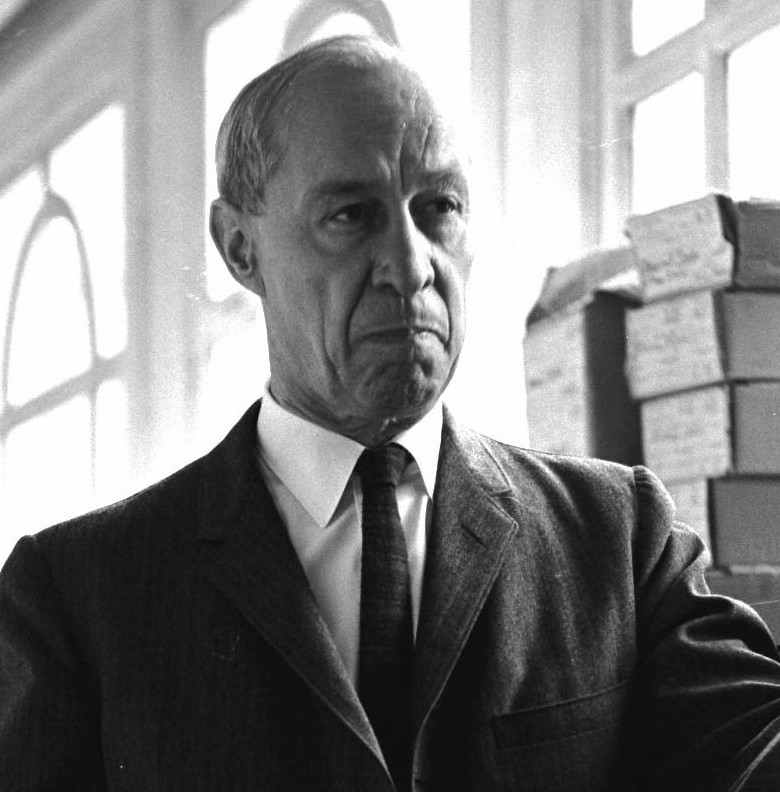
\includegraphics[width=\linewidth]{likert.jpg}
    \caption{Rensis Likert (1903--1981)}
  \end{figure}
  \column{0.45\textwidth}
  \begin{block}{Likert Scale}
    \small
    The Likert scale, or \textit{summated rating scale}, is widely used because it is easy to construct: a series of statements (\textit{items}) semantically linked to the attitudes under study are considered, and batteries of questions are constructed in which the respondent is asked to express their degree of agreement or disagreement.
  \end{block}
\end{columns}
\end{frame}

\begin{frame}{Example: Neophobia towards food technologies}
  \begin{block}{Food Technology Neophobia Scale (Cox \& Evans, 2008)}
    The FTNS is a popular instrument for measuring neophobia towards food technologies and is based on the Likert scale.
  \end{block}
  \vspace{0.3cm}
  \small
  \begin{tabular}{l l}
    \textbf{FTNS 1:} & I don't need to eat food made using new technology \\
    & because the food I already eat is fine \\
    \textbf{FTNS 2:} & New food technologies are something I am \\
    & uncertain about \\
    \textbf{FTNS 3:} & New food products are not healthier than \\
    & traditional foods \\
    \textbf{(...)}
  \end{tabular}
  \vspace{0.2cm}
  \begin{center}
    \footnotesize
    \begin{tabular}{ccccc}
      \toprule
      \textit{Strongly} & \textit{Disagree} & \textit{Neither agree} & \textit{Agree} & \textit{Strongly} \\
      \textit{disagree} &  & \textit{nor disagree} &  & \textit{agree} \\
      \midrule
      $\bigcirc$ & $\bigcirc$ & $\bigcirc$ & $\bigcirc$ & $\bigcirc$ \\
      \bottomrule
    \end{tabular}
  \end{center}
\end{frame}

\begin{frame}{Example: Neophobia towards food technologies}
  \begin{block}{Food Technology Neophobia Scale (Cox \& Evans, 2008)}
    The FTNS is a popular instrument for measuring aversion to new food technologies and is based on the Likert scale.
  \end{block}
  \vspace{0.3cm}
  \small
  \begin{tabular}{l l}
    \textbf{FTNS 1:} & I don't need to eat food made using new technology \\
    & because the food I already eat is fine \\
    \textbf{FTNS 2:} & New food technologies are something I am \\
    & uncertain about \\
    \textbf{FTNS 3:} & New food products are not healthier than \\
    & traditional foods \\
    \textbf{(...)}
  \end{tabular}
  \vspace{0.2cm}
  \begin{center}
    \footnotesize
    \begin{tabular}{ccccc}
      \toprule
      \textit{Strongly} & \textit{Disagree} & \textit{Neither agree} & \textit{Agree} & \textit{Strongly} \\
      \textit{disagree} &  & \textit{nor disagree} &  & \textit{agree} \\
      \midrule
      1 & 2 & 3 & 4 & 5 \\
      \bottomrule
    \end{tabular}
  \end{center}
\end{frame}

\begin{frame}{Measuring attitudes: Semantic Differential}
\begin{columns}[c]
  \column{0.55\textwidth}
  \begin{figure}
    \centering
    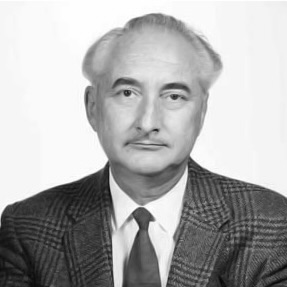
\includegraphics[width=\linewidth]{osgood.jpg}
    \caption{Charles E. Osgood (1916--1991)}
  \end{figure}
  \column{0.45\textwidth}
  \begin{block}{Osgood Scale}
    \small
    The Osgood scale, or \textit{semantic differential}, is based on pairs of opposite adjectives. The respondent indicates their position along a continuum, thus revealing their mental representation of the target concept.
  \end{block}
\end{columns}
\end{frame}

\begin{frame}{Example target: ``Stata''}
  \begin{center}
    \small
    \begin{tabular}{|c|c|c|c|c|c|c|c|c|}
    \hline
      & -3 & -2 & -1 & 0 & 1 & 2 & 3 & \\
      \hline
      \text{Aggressive} & $\bigcirc$ & $\bigcirc$ & $\bigcirc$ & $\bigcirc$ & $\bigcirc$ & $\bigcirc$ & $\bigcirc$ & \text{Peaceful} \\
      \hline
      \text{Unpleasant}  & $\bigcirc$ & $\bigcirc$ & $\bigcirc$ & $\bigcirc$ & $\bigcirc$ & $\bigcirc$ & $\bigcirc$ & \text{Pleasant} \\
      \hline
      \text{...} & $\bigcirc$ & $\bigcirc$ & $\bigcirc$ & $\bigcirc$ & $\bigcirc$ & $\bigcirc$ & $\bigcirc$ & \text{...} \\
      \hline
    \end{tabular}
  \end{center}
  \pause
  \begin{figure}
    \centering
    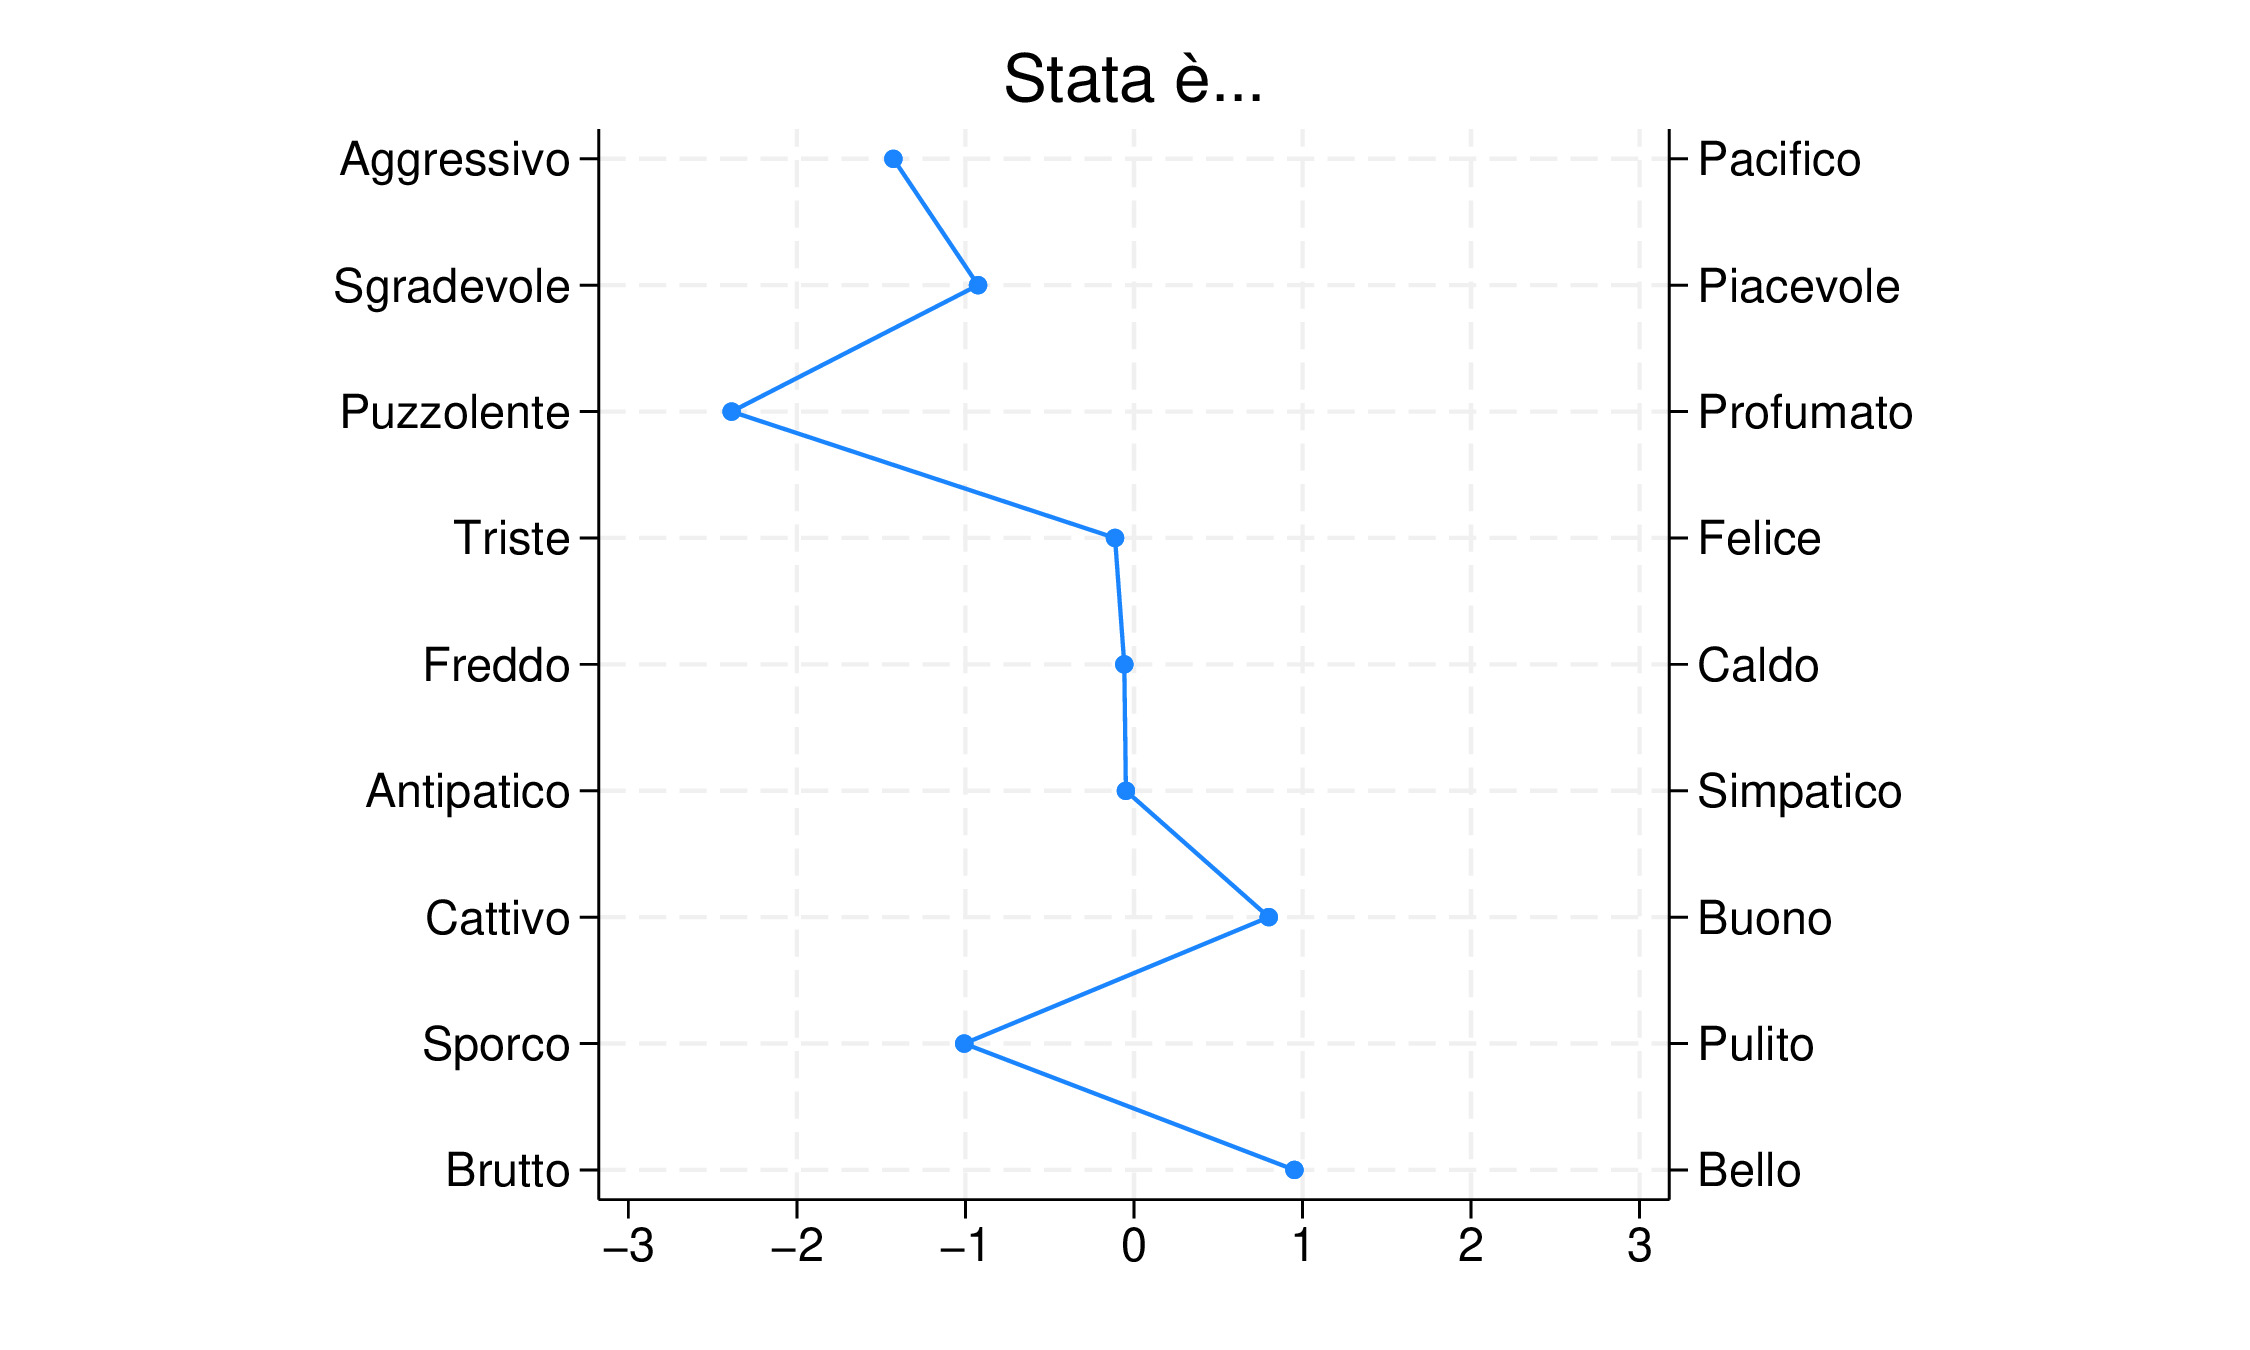
\includegraphics[width=0.9\linewidth]{osgood_stata.jpg}
  \end{figure}
\end{frame}

\end{document}
